%
% ---------------------------------------------------------------
% Copyright (C) 2012-2018 Gang Li
% ---------------------------------------------------------------
%
% This work is the default powerdot-tuliplab style test file and may be
% distributed and/or modified under the conditions of the LaTeX Project Public
% License, either version 1.3 of this license or (at your option) any later
% version. The latest version of this license is in
% http://www.latex-project.org/lppl.txt and version 1.3 or later is part of all
% distributions of LaTeX version 2003/12/01 or later.
%
% This work has the LPPL maintenance status "maintained".
%
% This Current Maintainer of this work is Gang Li.
%
%

\documentclass[
 size=14pt,
 paper=smartboard,  %a4paper, smartboard, screen
 mode=present, 		%present, handout, print
 display=slides, 	% slidesnotes, notes, slides
 style=tuliplab,  	% TULIP Lab style
 pauseslide,
 fleqn,leqno]{powerdot}


\usepackage{cancel}
\usepackage{caption}
\usepackage{stackengine}
\usepackage{smartdiagram}
\usepackage{attrib}
\usepackage{amssymb}
\usepackage{amsmath} 
\usepackage{amsthm} 
\usepackage{mathtools}
\usepackage{rotating}
\usepackage{graphicx}

\usepackage{boxedminipage}
\usepackage{rotate}
\usepackage{calc}
\usepackage[absolute]{textpos}
\usepackage{psfrag,overpic}
\usepackage{fouriernc}
\usepackage{pstricks,pst-3d,pst-grad,pstricks-add,pst-text,pst-node,pst-tree}
\usepackage{moreverb,epsfig,subfigure}
\usepackage{color}
\usepackage{booktabs}
\usepackage{etex}
\usepackage{breqn}
\usepackage{multirow}
\usepackage{natbib}
\usepackage{bibentry}
\usepackage{gitinfo2}
\usepackage{siunitx}
\usepackage{nicefrac}
%\usepackage{geometry}
%\geometry{verbose,letterpaper}
\usepackage{media9}
\usepackage{animate}
%\usepackage{movie15}
\usepackage{auto-pst-pdf}

\usepackage{breakurl}
\usepackage{fontawesome}
\usepackage{xcolor}
\usepackage{multicol}



\usepackage{verbatim}
\usepackage[utf8]{inputenc}
\usepackage{dtk-logos}
\usepackage{tikz}
\usepackage{adigraph}
%\usepackage{tkz-graph}
\usepackage{hyperref}
%\usepackage{ulem}
\usepackage{pgfplots}
\usepackage{verbatim}
\usepackage{fontawesome}


\usepackage{todonotes}
% \usepackage{pst-rel-points}
\usepackage{animate}
\usepackage{fontawesome}

\usepackage{listings}
\lstset{frameround=fttt,
frame=trBL,
stringstyle=\ttfamily,
backgroundcolor=\color{yellow!20},
basicstyle=\footnotesize\ttfamily}
\lstnewenvironment{code}{
\lstset{frame=single,escapeinside=`',
backgroundcolor=\color{yellow!20},
basicstyle=\footnotesize\ttfamily}
}{}


\usepackage{hyperref}
\hypersetup{ % TODO: PDF meta Data
  pdftitle={Presentation Title},
  pdfauthor={Gang Li},
  pdfpagemode={FullScreen},
  pdfborder={0 0 0}
}


% \usepackage{auto-pst-pdf}
% package to show source code

\definecolor{LightGray}{rgb}{0.9,0.9,0.9}
\newlength{\pixel}\setlength\pixel{0.000714285714\slidewidth}
\setlength{\TPHorizModule}{\slidewidth}
\setlength{\TPVertModule}{\slideheight}
\newcommand\highlight[1]{\fbox{#1}}
\newcommand\icite[1]{{\footnotesize [#1]}}

\newcommand\twotonebox[2]{\fcolorbox{pdcolor2}{pdcolor2}
{#1\vphantom{#2}}\fcolorbox{pdcolor2}{white}{#2\vphantom{#1}}}
\newcommand\twotoneboxo[2]{\fcolorbox{pdcolor2}{pdcolor2}
{#1}\fcolorbox{pdcolor2}{white}{#2}}
\newcommand\vpspace[1]{\vphantom{\vspace{#1}}}
\newcommand\hpspace[1]{\hphantom{\hspace{#1}}}
\newcommand\COMMENT[1]{}

\newcommand\placepos[3]{\hbox to\z@{\kern#1S
        \raisebox{-#2}[\z@][\z@]{#3}\hss}\ignorespaces}

\renewcommand{\baselinestretch}{1.2}


\newcommand{\draftnote}[3]{
	\todo[author=#2,color=#1!30,size=\footnotesize]{\textsf{#3}}	}
% TODO: add yourself here:
%
\newcommand{\gangli}[1]{\draftnote{blue}{GLi:}{#1}}
\newcommand{\shaoni}[1]{\draftnote{green}{sn:}{#1}}
\newcommand{\gliMarker}
	{\todo[author=GLi,size=\tiny,inline,color=blue!40]
	{Gang Li has worked up to here.}}
\newcommand{\snMarker}
	{\todo[author=Sn,size=\tiny,inline,color=green!40]
	{Shaoni has worked up to here.}}

%%%%%%%%%%%%%%%%%%%%%%%%%%%%%%%%%%%%%%%%%%%%%%%%%%%%%%%%%%%%%%%%%%%%%%%%
% title
% TODO: Customize to your Own Title, Name, Address
%
\title{The mid-term report}
\author{
   Jincai Ma
\\
\\Xi'an Shiyou University}
\date{\today}


% Customize the setting of slides
\pdsetup{
% TODO: Customize the left footer, and right footer
rf=\href{http://www.tulip.org.au}{
Last Changed by: \textsc{\gitCommitterName}\ \gitVtagn-\gitAbbrevHash\ (\gitAuthorDate)
},
cf={The mid-term report},
}


\begin{document}

\maketitle

%\begin{slide}{Overview}
%\tableofcontents[content=sections]
%\end{slide}


%%==========================================================================================




%%==========================================================================================
%%
\begin{slide}{Introduction}
\begin{center}

{
\begin{itemize}
\item 
The bike-sharing system is a way to rent bikes through a city-wide network of kiosk locations, automatically gaining membership, renting and returning bikes.People can rent a bike from one place and return it to another as needed.
\item Historical car records combine date, weather, temperature, humidity and other factors to predict the bike-sharing program needs in Washington.

\end{itemize}
}

\end{center}
\bigskip
\begin{center}

\end{center}
\bigskip

%%==========================================================================================

%%==========================================================================================

\end{slide}
%%
%%==========================================================================================



%%
\begin{slide}{Data Description}
  \begin{center}

    {
      \begin{itemize}
        \item
        Descriptive statistics of the data
      \end{itemize}  
      \begin{figure}
        \centering
        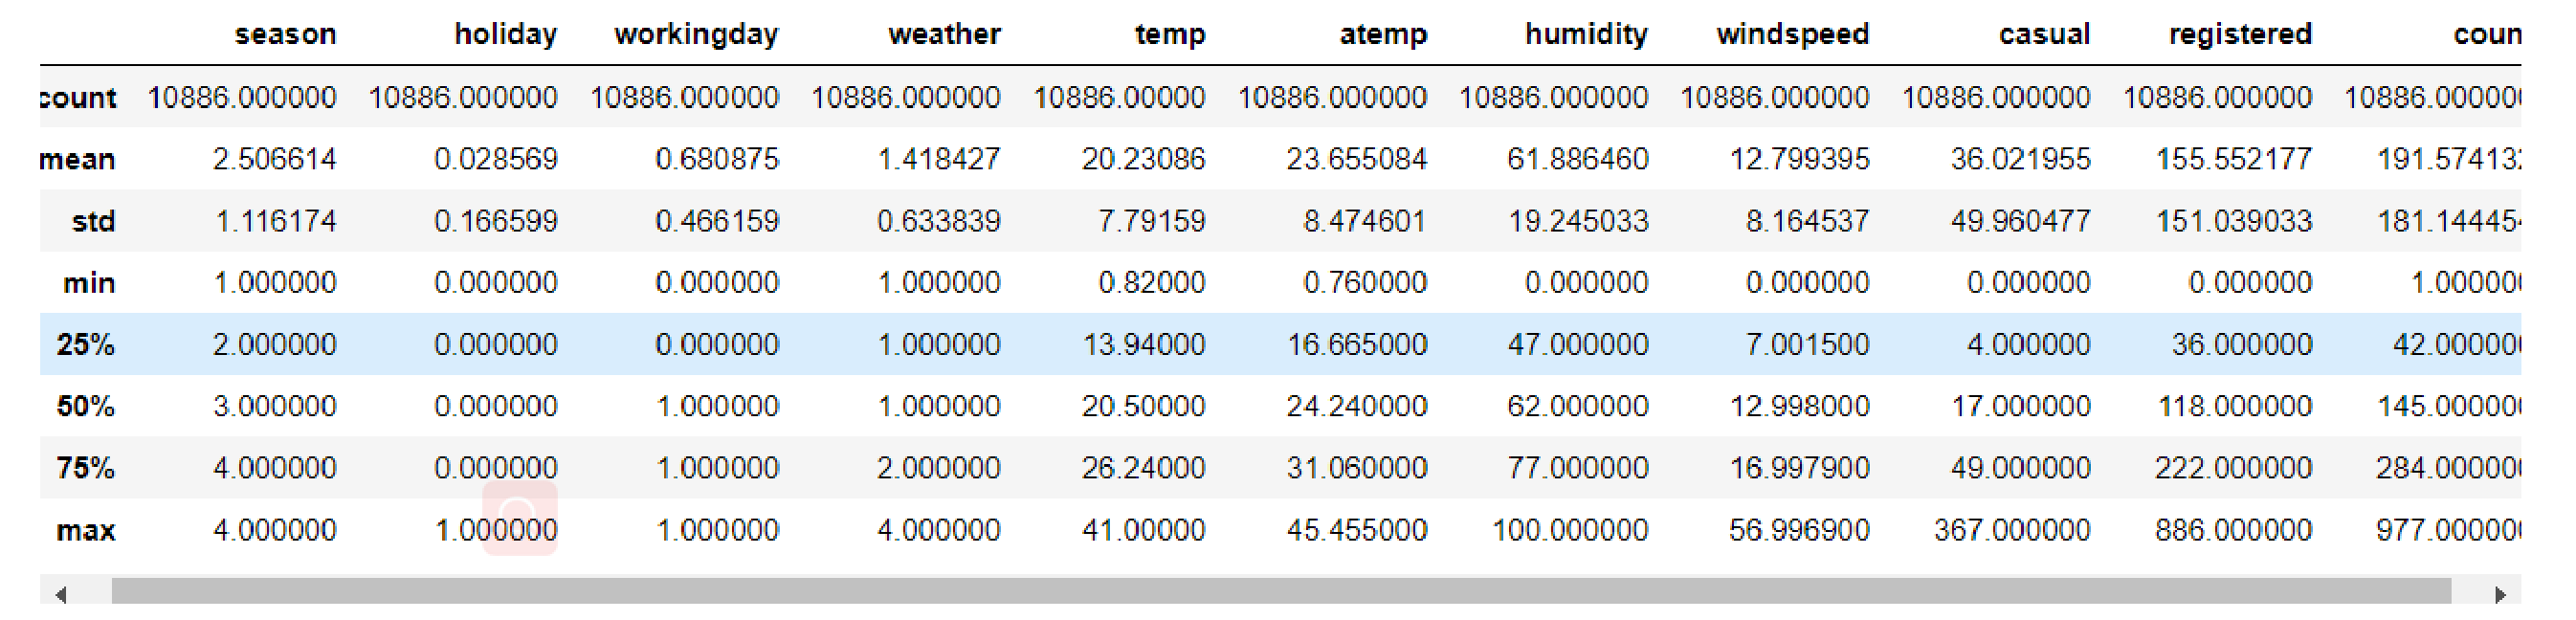
\includegraphics[width=0.9\textwidth]{pic/a.eps}
     
      \end{figure}
    

        
       
    }
    \end{center}
    \bigskip
    \begin{center}
    
    \end{center}
    \bigskip

%%==========================================================================================


%%==========================================================================================
\end{slide}
%%
%%==========================================================================================

%%==========================================================================================
%%
\begin{slide}{Data  Visualization}
  \begin{center}

    {
      \begin{itemize}
      
        \item The standard deviation of the number of leases you have to predict at the end is very large.So let's look at the distribution by drawing it.
      \end{itemize} 
      \begin{figure}
        \centering
        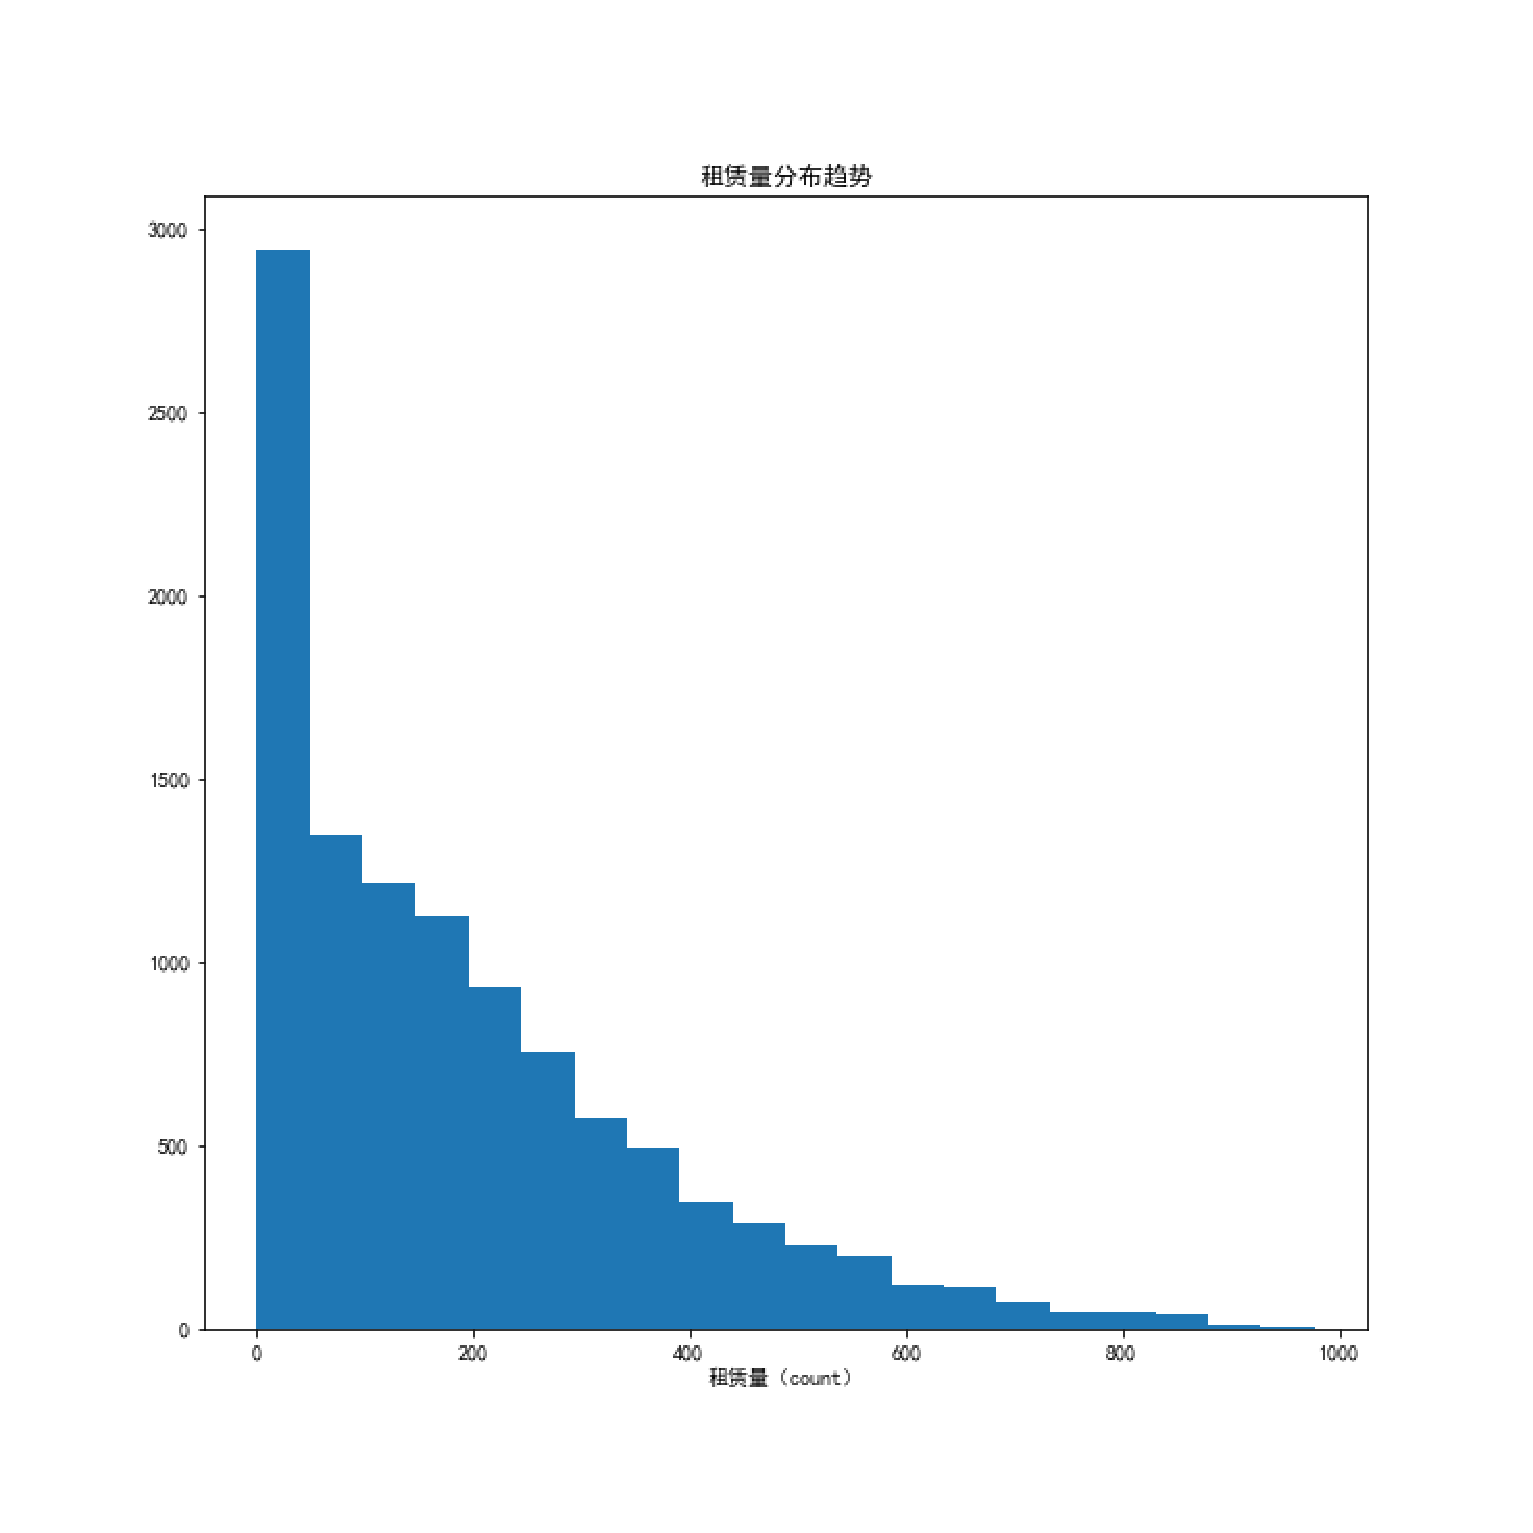
\includegraphics[width=0.4\textwidth]{pic/count .eps} 
      \end{figure}
    

        
       
    }
    \end{center}
  \bigskip
    \begin{center}
    
    \end{center}
  \bigskip



\end{slide}
%%
%%==========================================================================================
%%
\begin{slide}[toc=,bm=]{Data  Visualization}
  \begin{center}

    {
      \begin{itemize}
        \item Exclude data other than three standards,log of count
      \end{itemize} 
      \begin{figure}
        \centering
        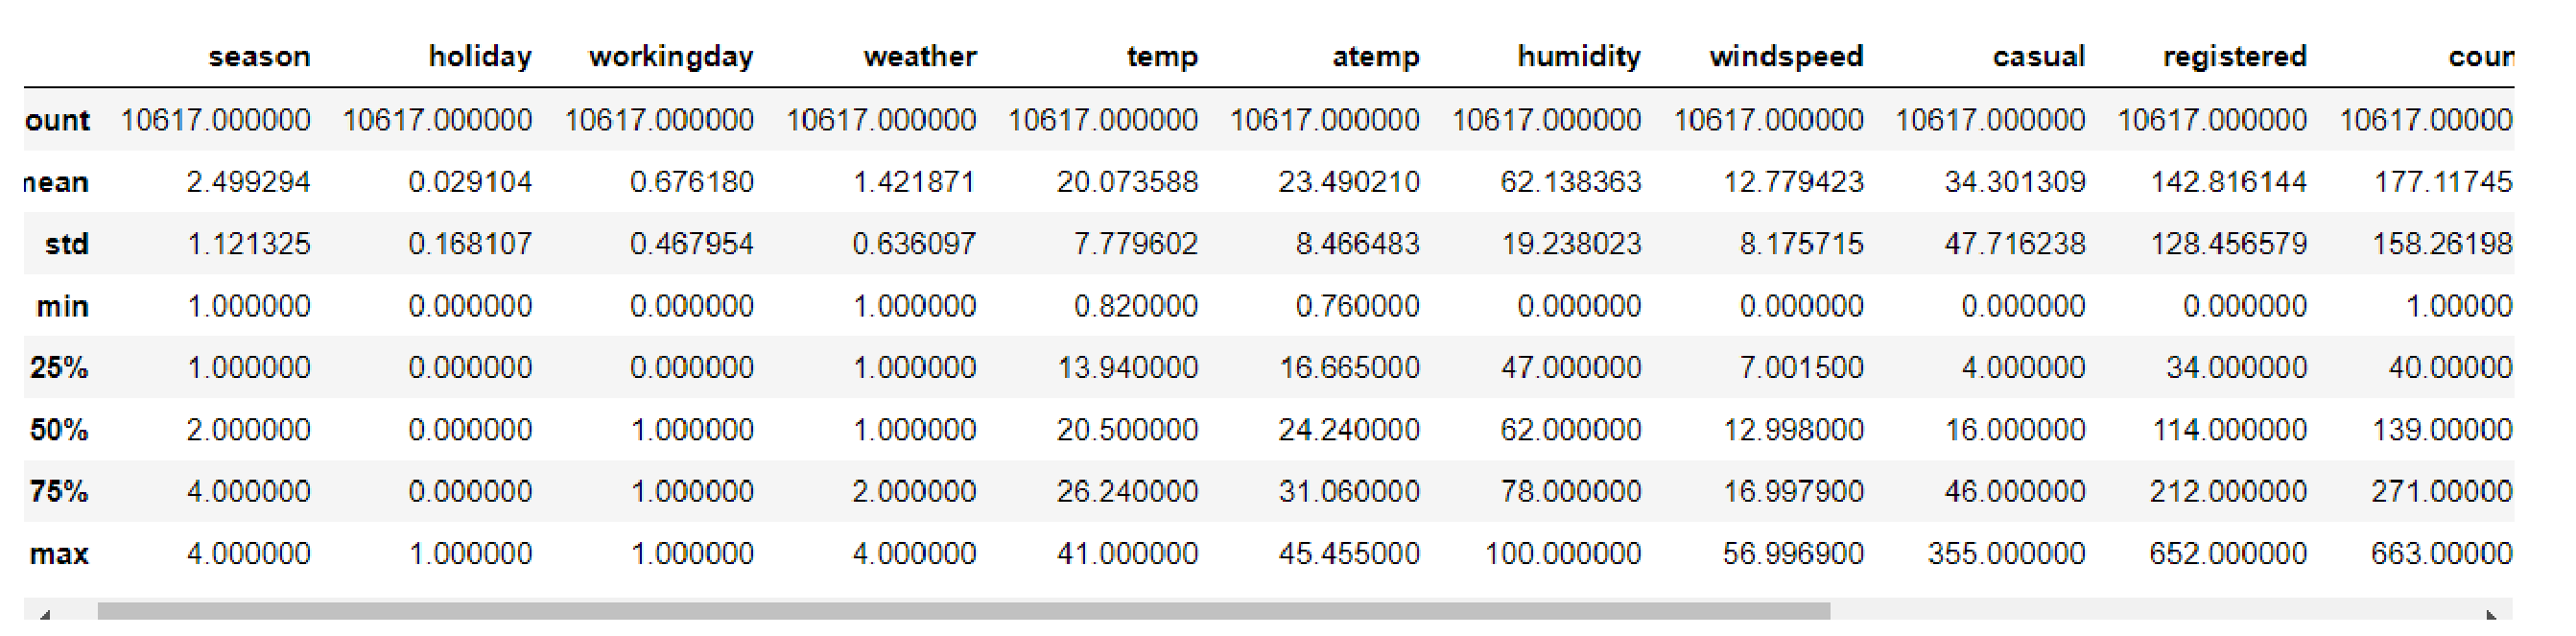
\includegraphics[width=0.8\textwidth]{pic/b.eps}
        \centering
        \begin{minipage}[t]{0.48\textwidth}
        \centering
        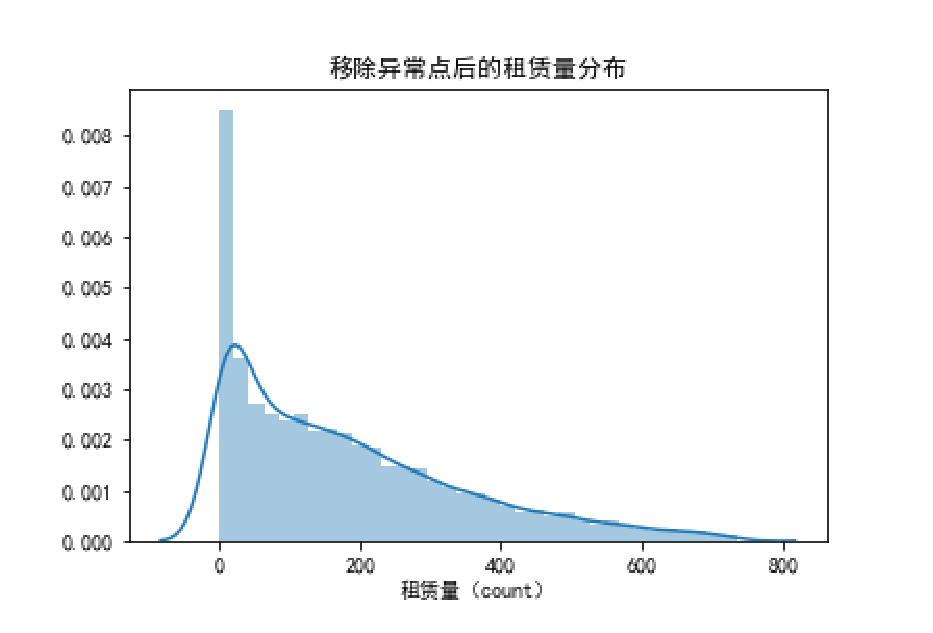
\includegraphics[width=0.9\textwidth]{pic/count a.eps}
        \end{minipage}
        \begin{minipage}[t]{0.48\textwidth}
        \centering
        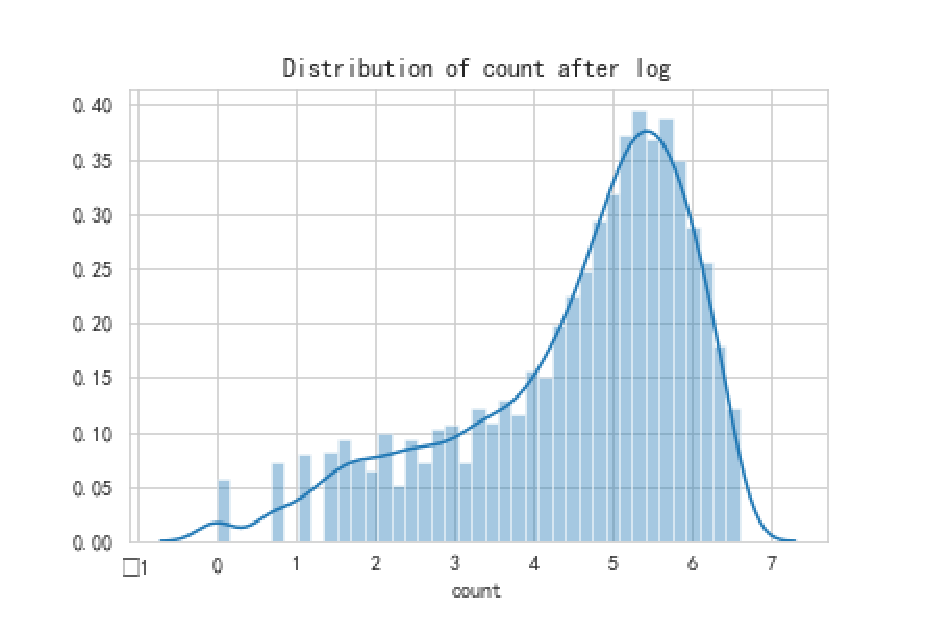
\includegraphics[width=0.9\textwidth]{pic/log.eps}
        \end{minipage}
      \end{figure}   
    }
    \end{center}
  


\end{slide}
%%
%%==========================================================================================
\begin{slide}[toc=,bm=]{Data  Visualization}
  \begin{center}

    {
      \begin{itemize}
          \item The impact of hour,month,season,year,weekday,workingday
      \end{itemize} 
        \begin{figure}
          \centering
          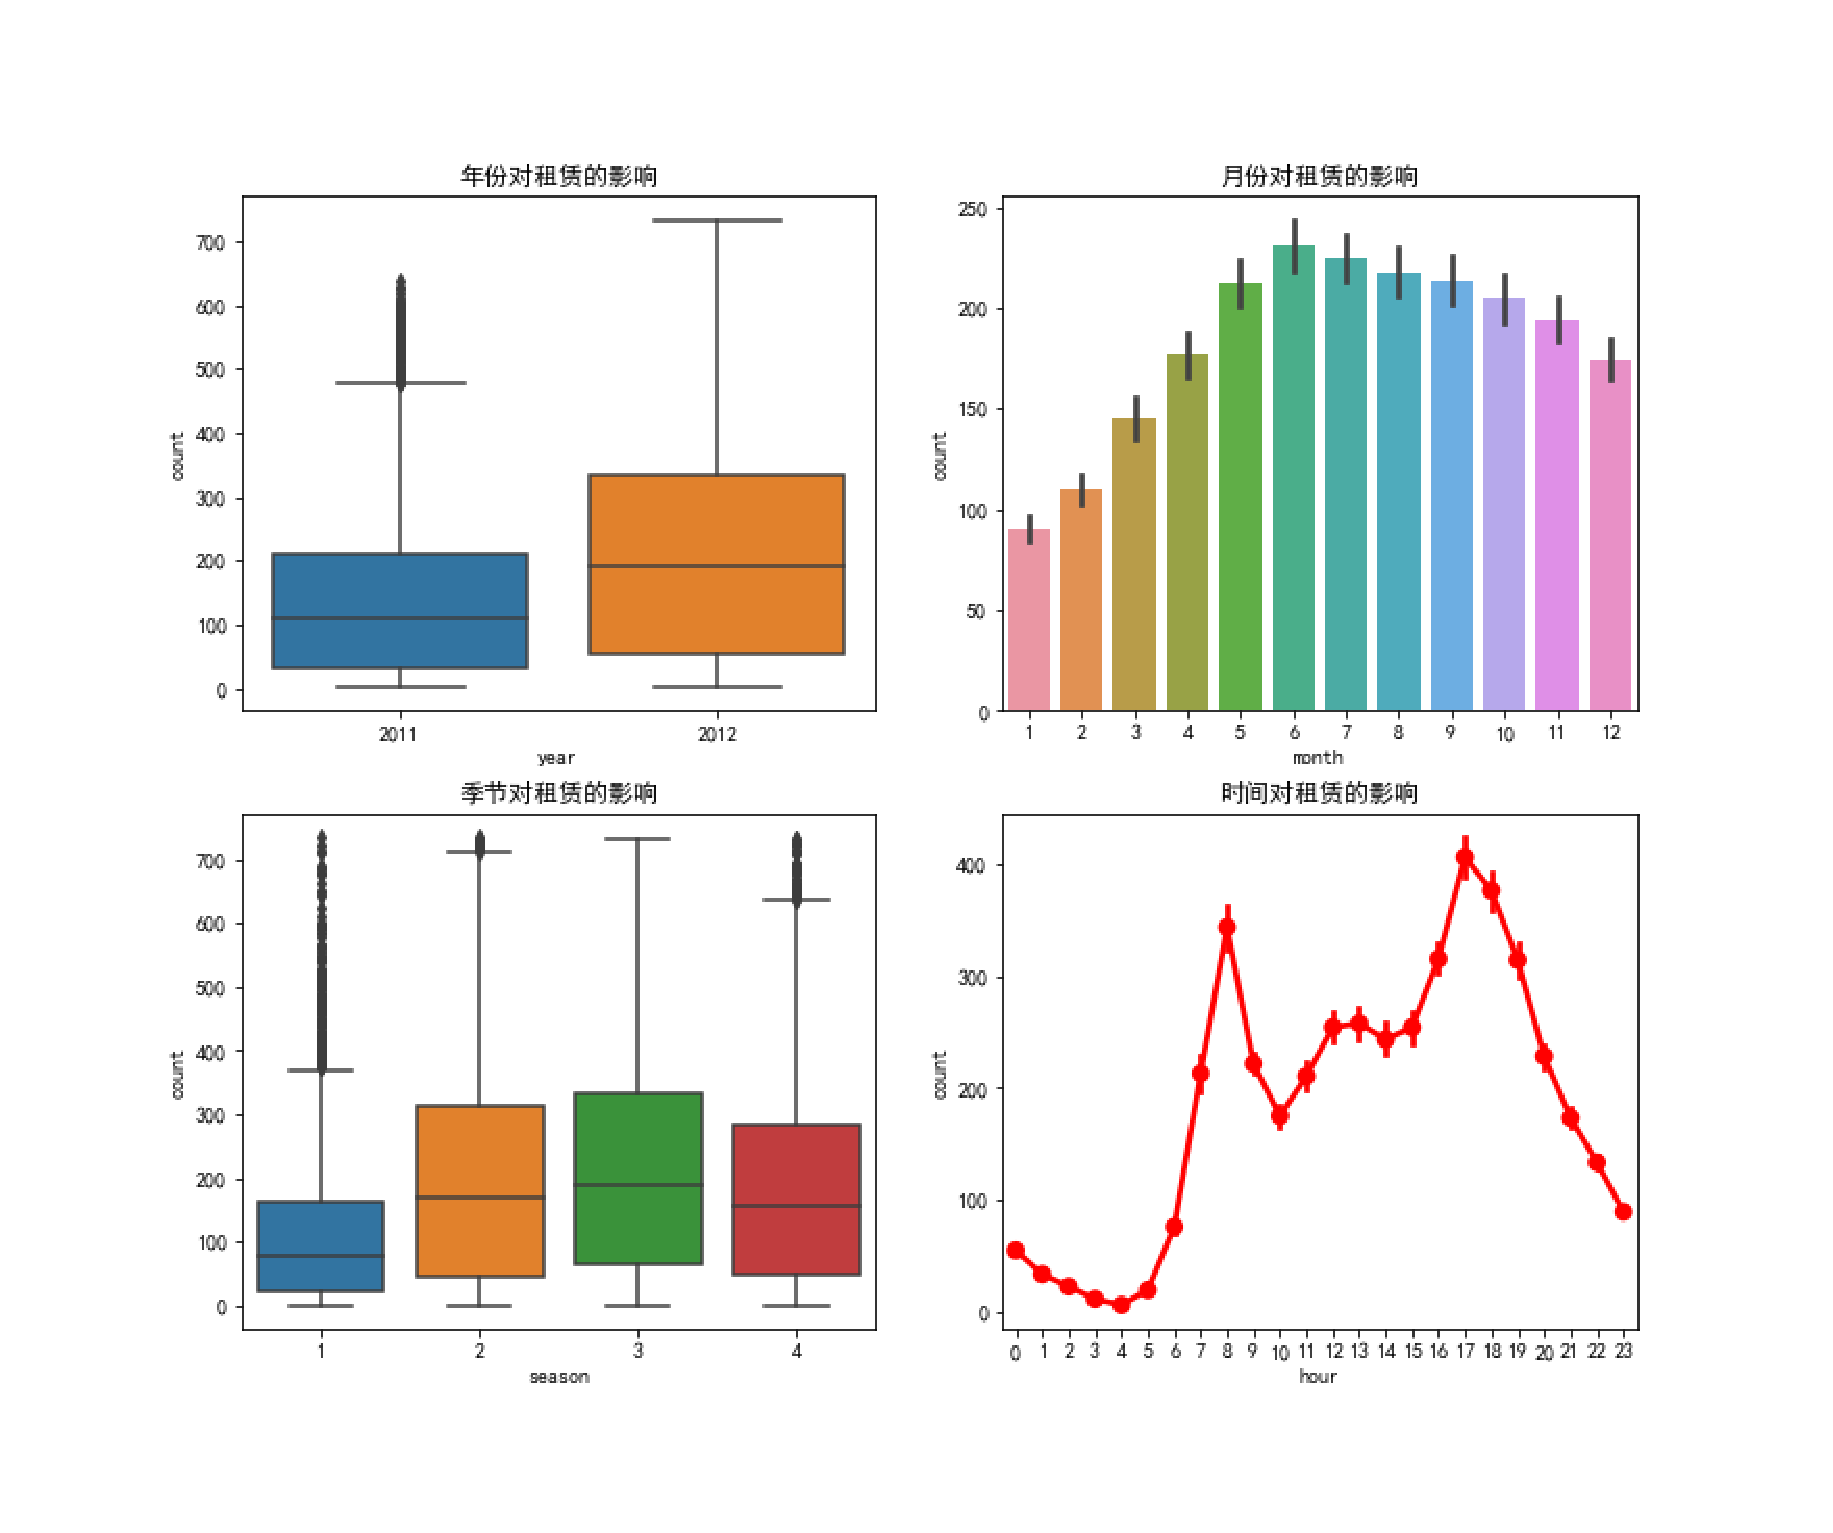
\includegraphics[height=0.5\textwidth]{pic/count all.eps}
          \centering
        \end{figure} 
    }
    \end{center}
 


\end{slide}
%%
%%==========================================================================================
\begin{slide}[toc=,bm=]{Data  Visualization}
  \begin{center}

    {
      \begin{itemize}
        
          \item The impact of weather
      \end{itemize} 
        \begin{figure}
          \centering
          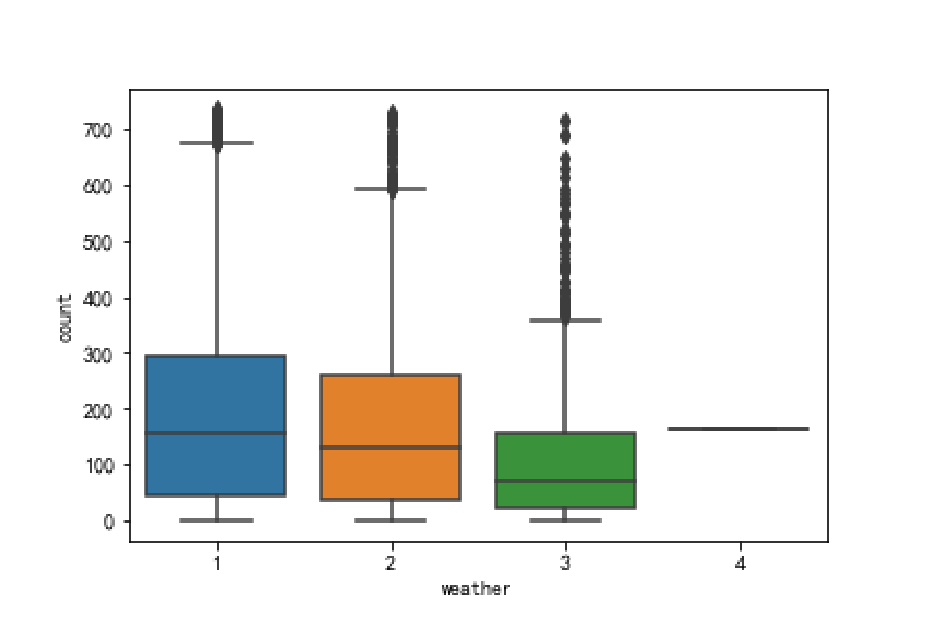
\includegraphics[width=0.5\textwidth]{pic/weather.eps}
          \centering
        \end{figure} 
    }
    \end{center}
 


\end{slide}
%%==========================================================================================
\begin{slide}[toc=,bm=]{Data  Visualization}
  \begin{center}

    {
      \begin{itemize}
        
          \item The impact of temp,atemp,humidity,windspeed
      \end{itemize} 
      \begin{figure}
        \centering
        \begin{minipage}[t]{0.45\textwidth}
        \centering
        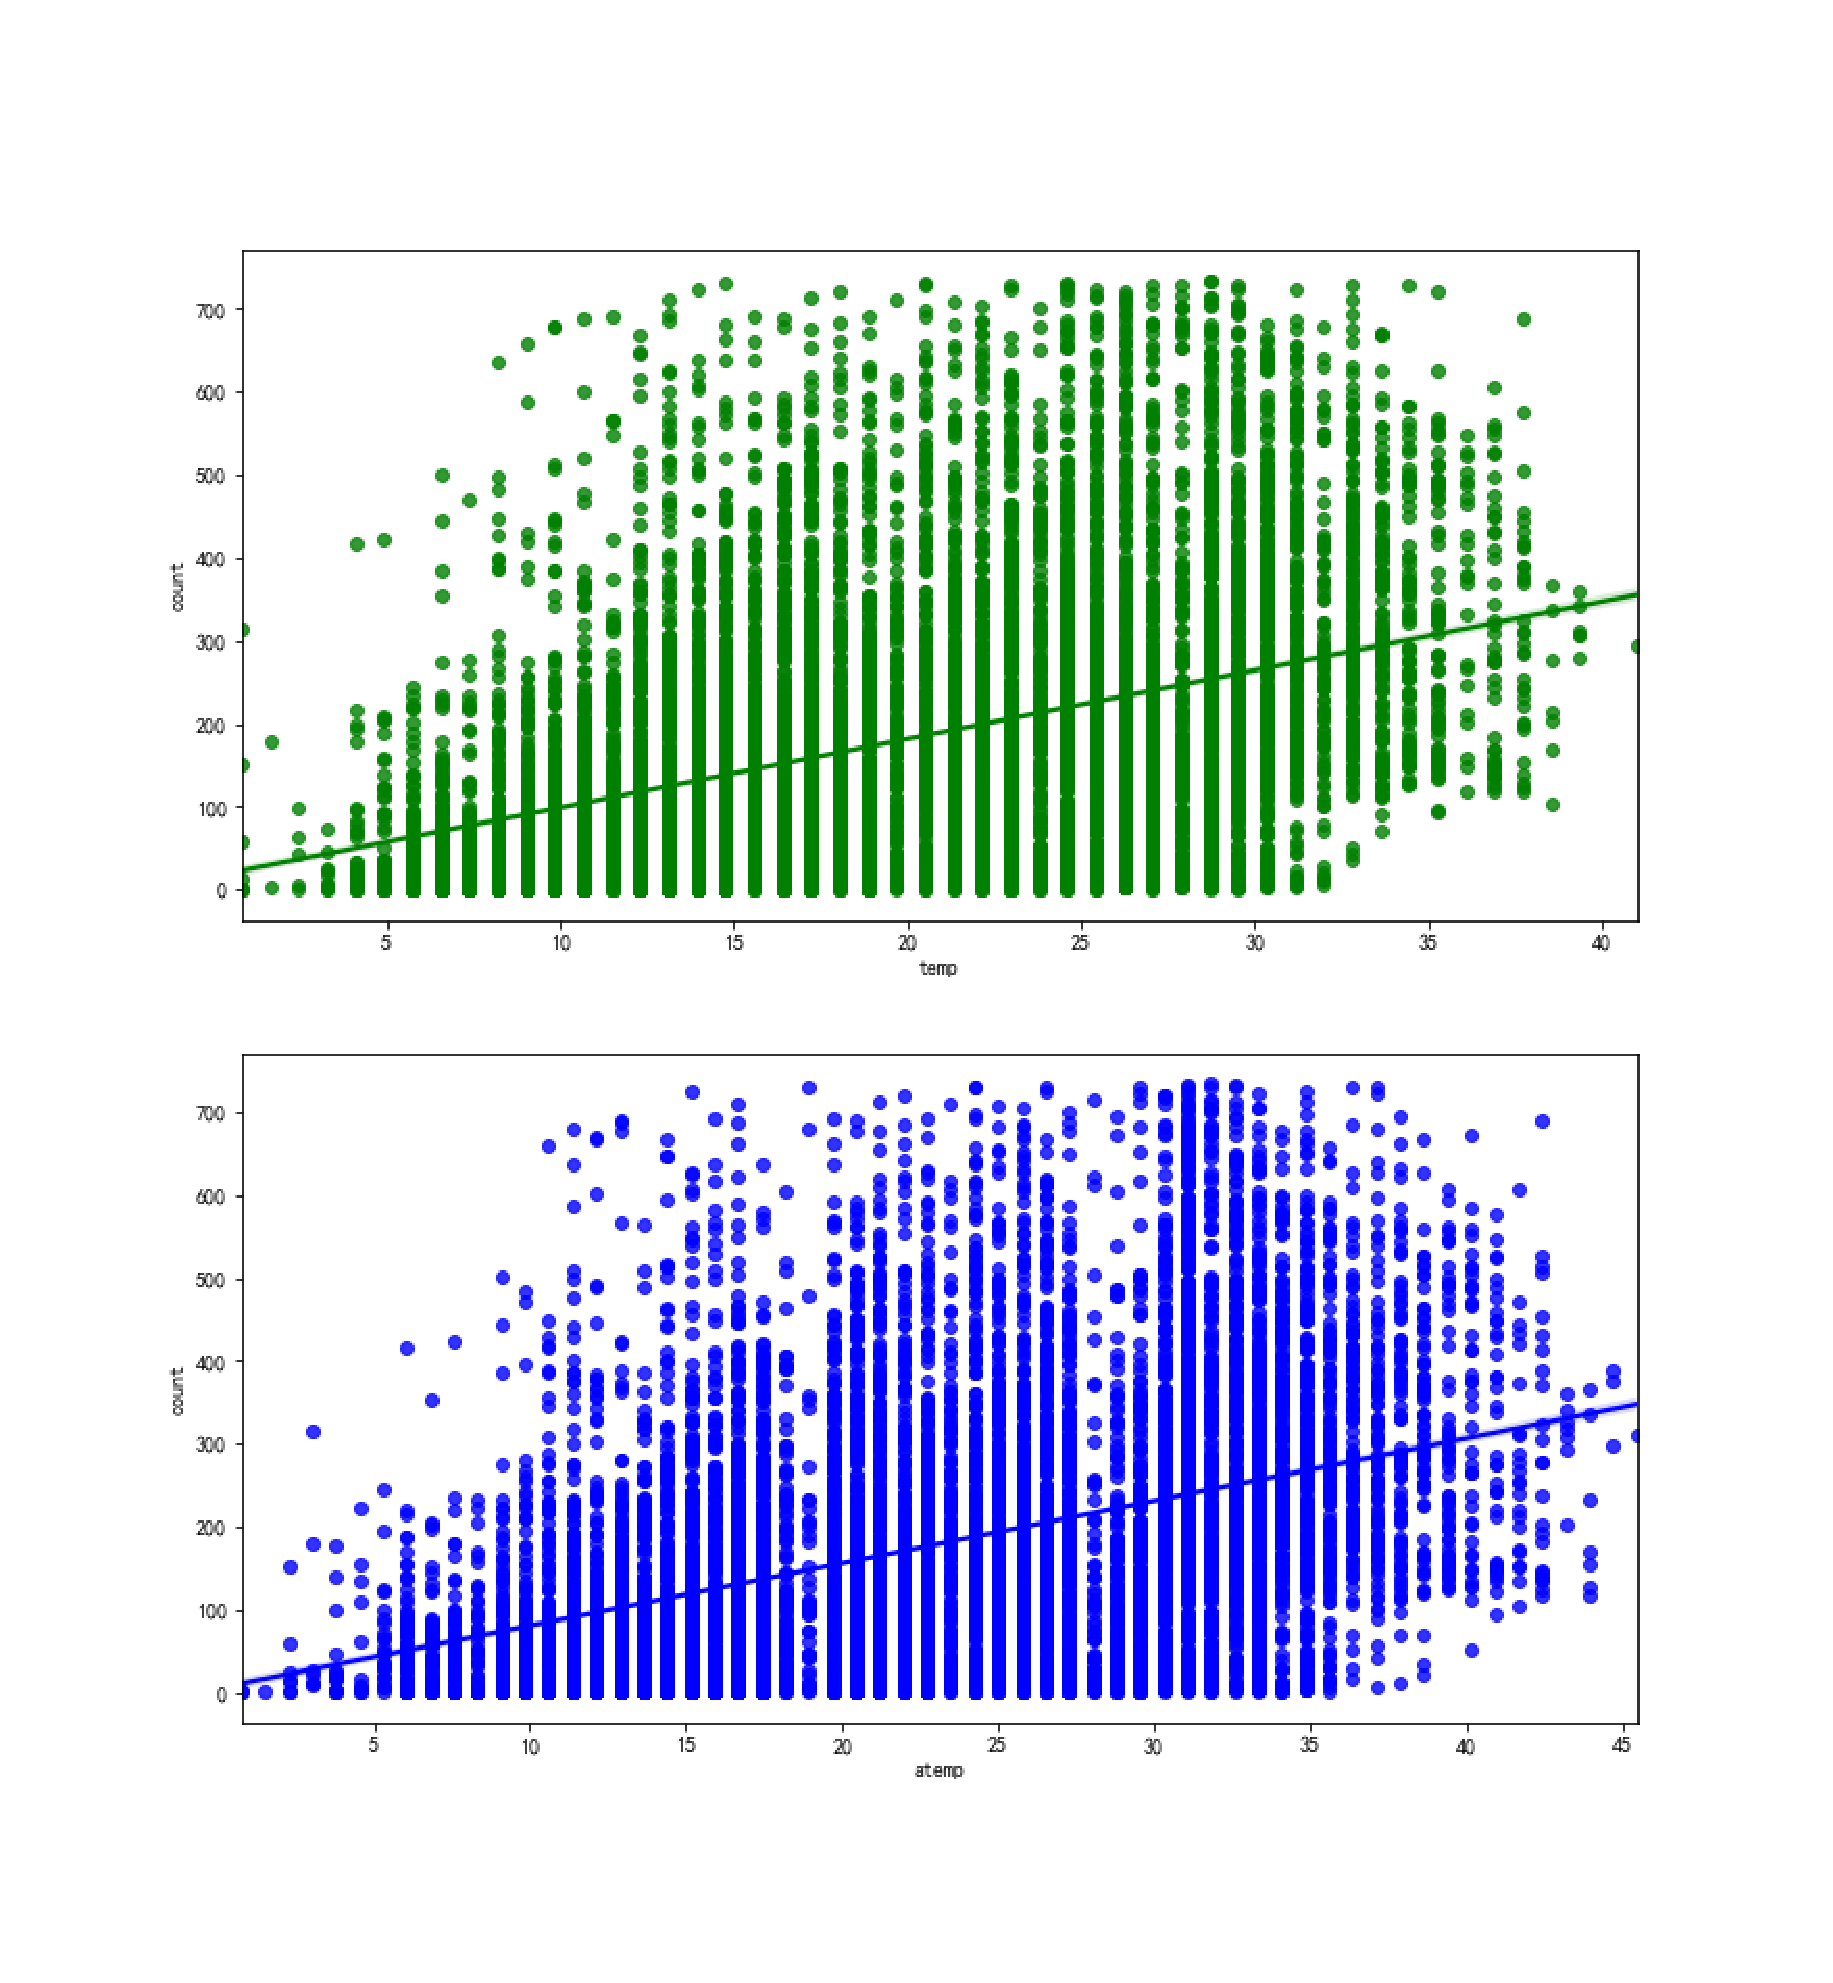
\includegraphics[width=1\textwidth]{pic/three tahw1.eps}
        \end{minipage}
        \begin{minipage}[t]{0.45\textwidth}
        \centering
        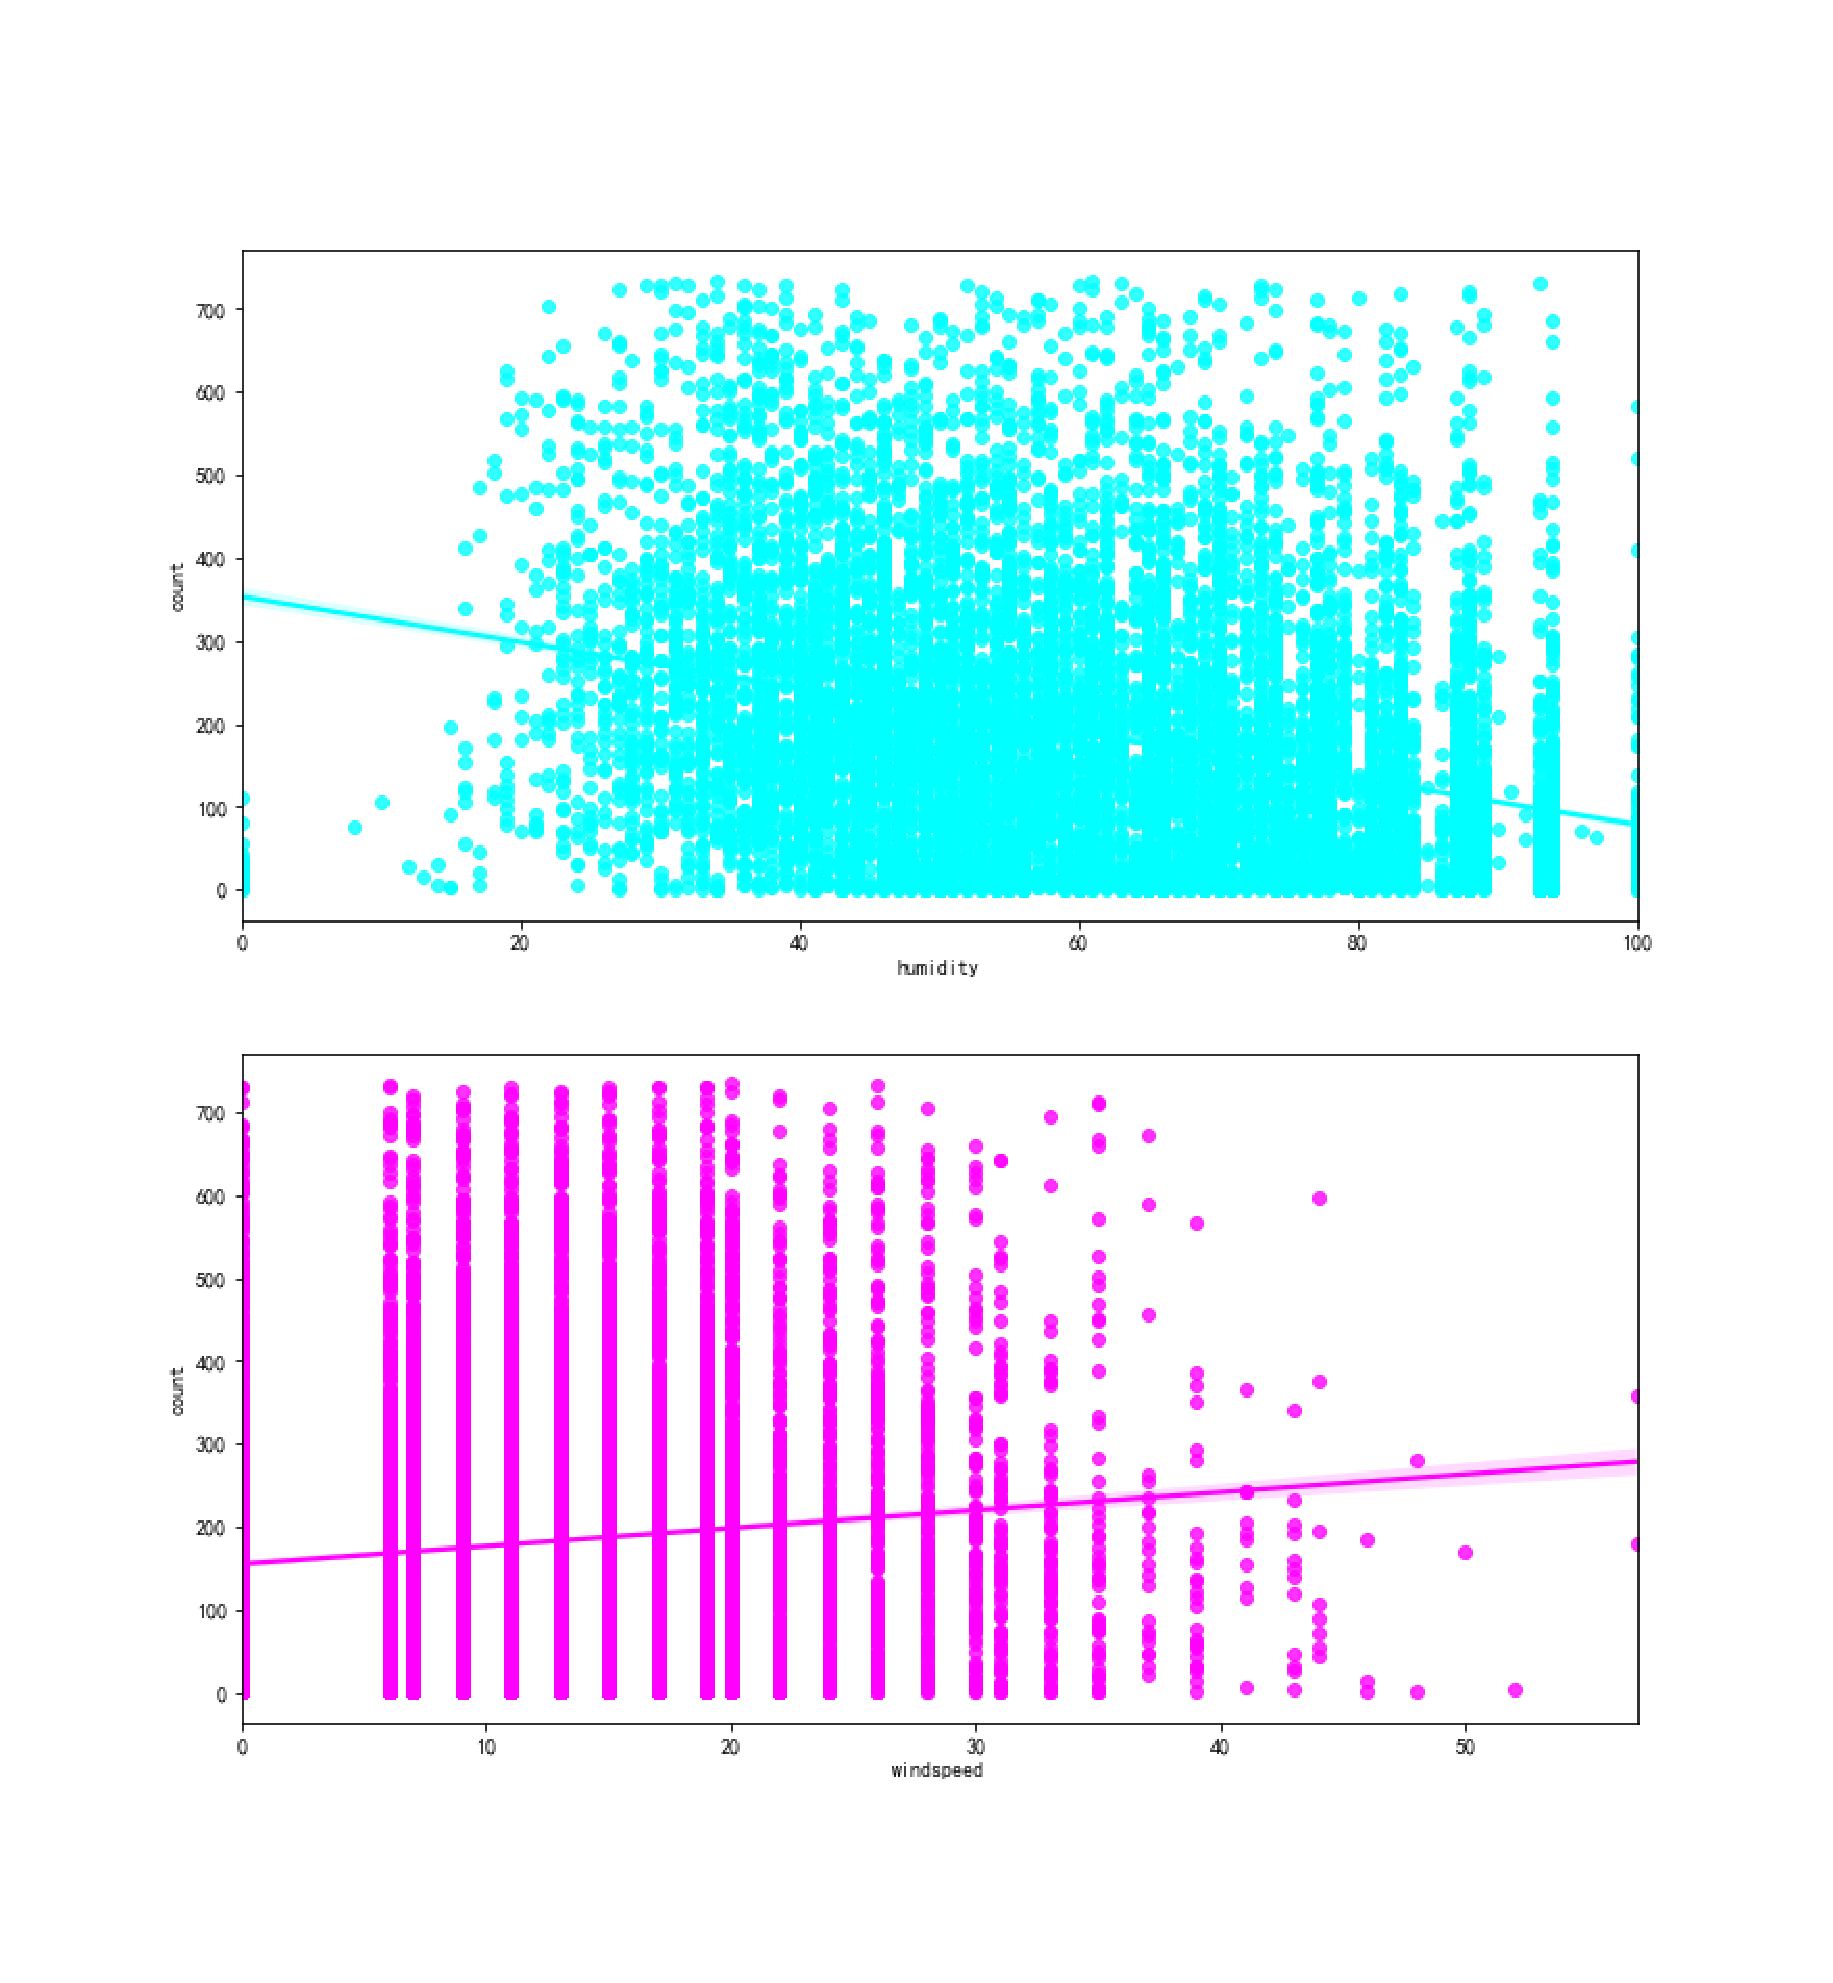
\includegraphics[width=1\textwidth]{pic/three tahw2.eps}
        \end{minipage}
      \end{figure}   
    }
    \end{center}
 


\end{slide}
%%==========================================================================================

%%==========================================================================================
\begin{slide}[toc=,bm=]{Data  Visualization}
  \begin{center}

    {
      \begin{itemize}
        
          \item Impact of season,week,registered and non-registered users on cycling usage trends
      \end{itemize} 
      \begin{itemize}
        
        \item For different times of the day, there is a clear trend in the use of Shared bikes, with two distinct peaks, in line with people's understanding of morning peak and evening peak.The trends were the same for all four seasons, except that usage in spring was slightly lower than in the other three.
    \end{itemize} 
      \begin{figure}
        \centering
        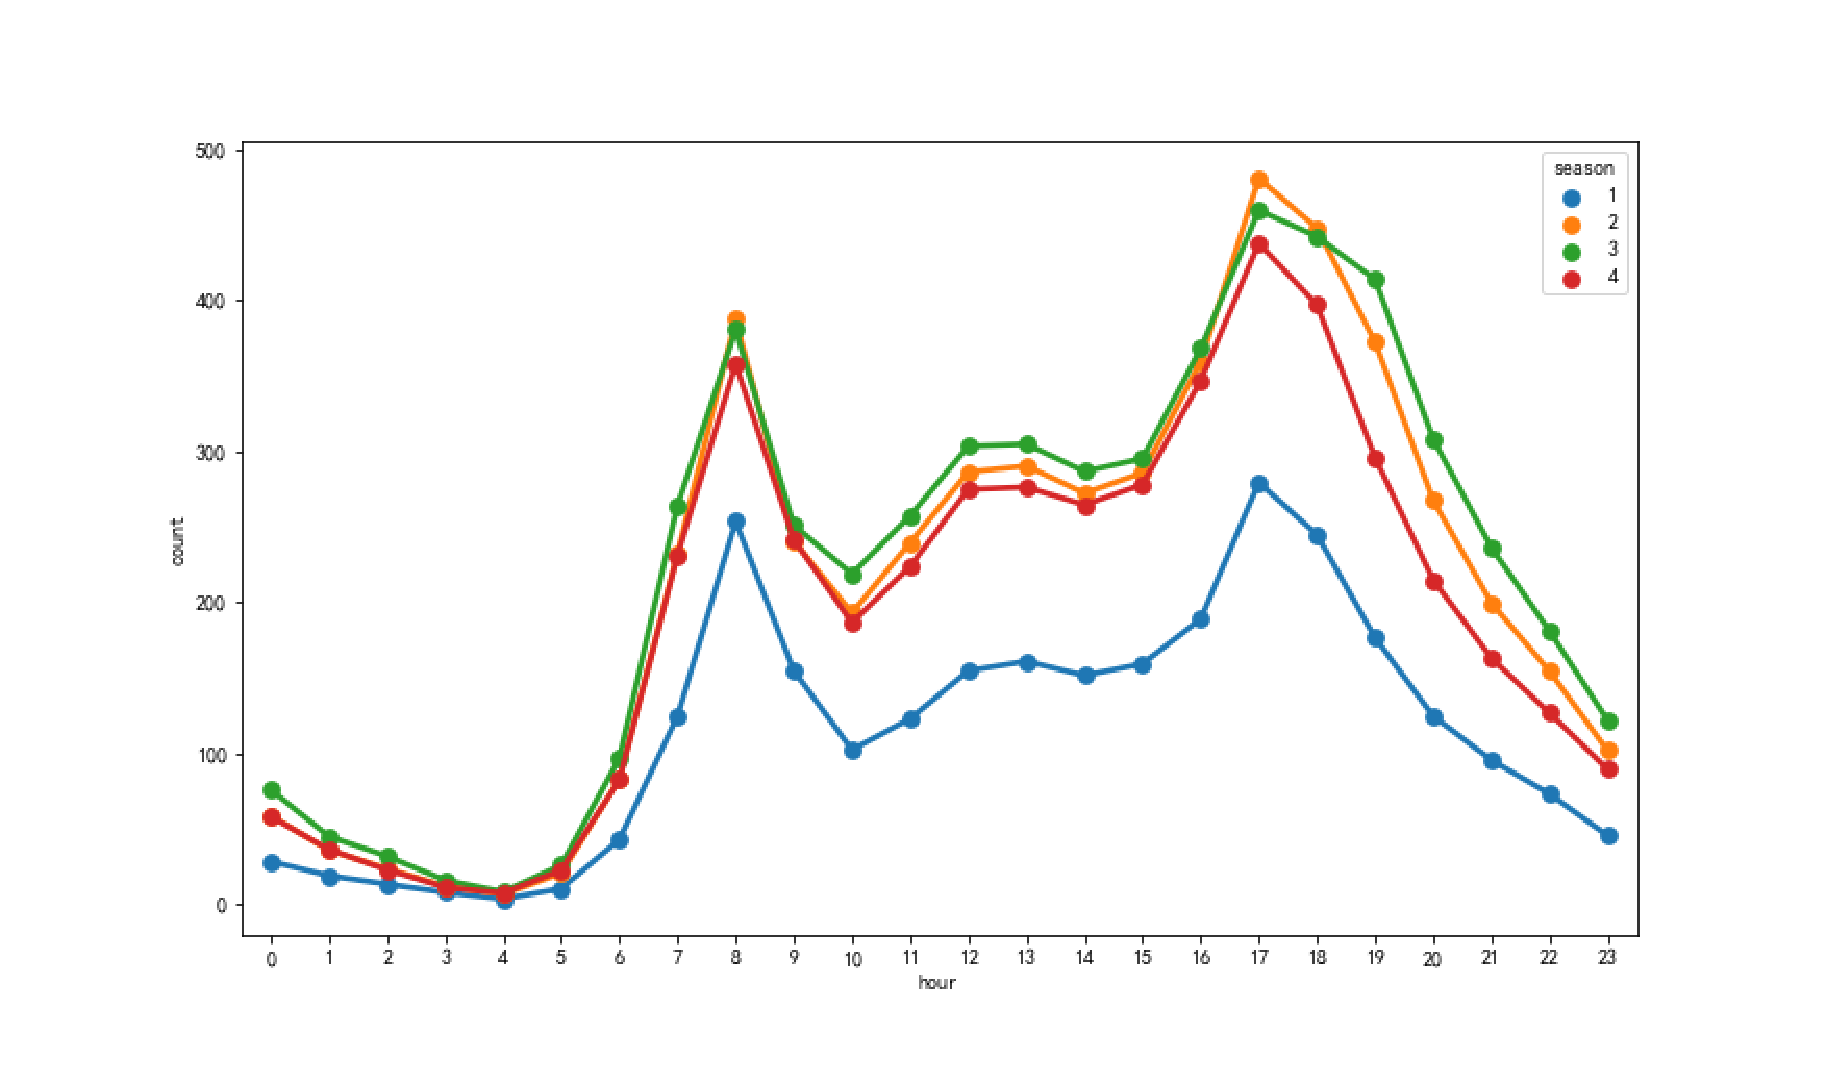
\includegraphics[width=0.5\textwidth]{pic/three hour1 (2).eps}
      \end{figure} 
      
     
    }
    \end{center}
 


\end{slide}
%%==========================================================================================
\begin{slide}[toc=,bm=]{Data  Visualization}
  \begin{center}

    {
      \begin{itemize}
        
        \item The usage of registered users accounts for the majority of the total usage, and the trend is consistent with the total usage trend, rather than that of registered users. The usage at different times of the day does not change much, and the trend is similar to the usage trend at weekends.
      \end{itemize} 
      \begin{figure}
        \centering
        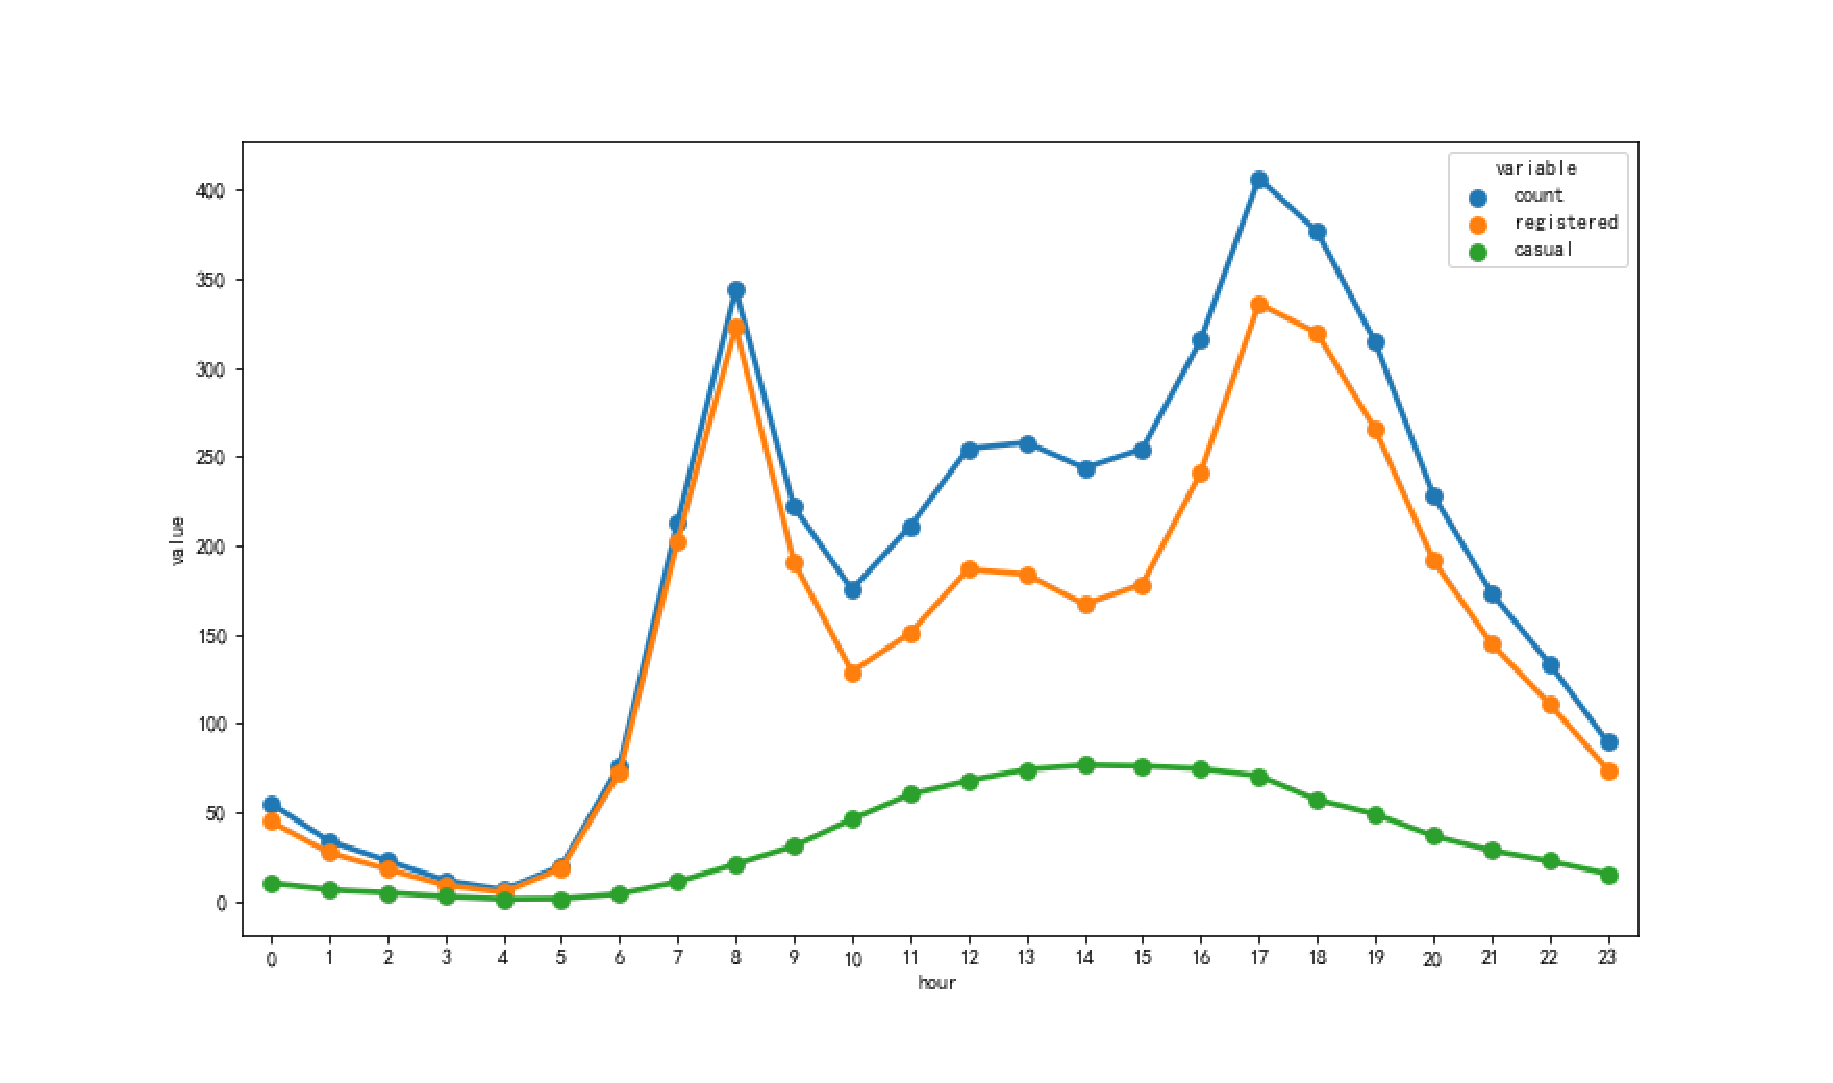
\includegraphics[width=0.5\textwidth]{pic/three hour3.eps}
      \end{figure}   
      
    }
    \end{center}
 


\end{slide}
%%==========================================================================================
\begin{slide}[toc=,bm=]{Data  Visualization}
  \begin{center}

    {
      \begin{itemize}
        
        \item From Monday to Friday, there are two peak usage periods, while on weekends, the usage trend is completely different from that on weekdays. The usage trend changes from bimodal to flat unimodal, and the peak usage period is concentrated at 11-17 o 'clock.
    \end{itemize}   
      \begin{figure}
        \centering
        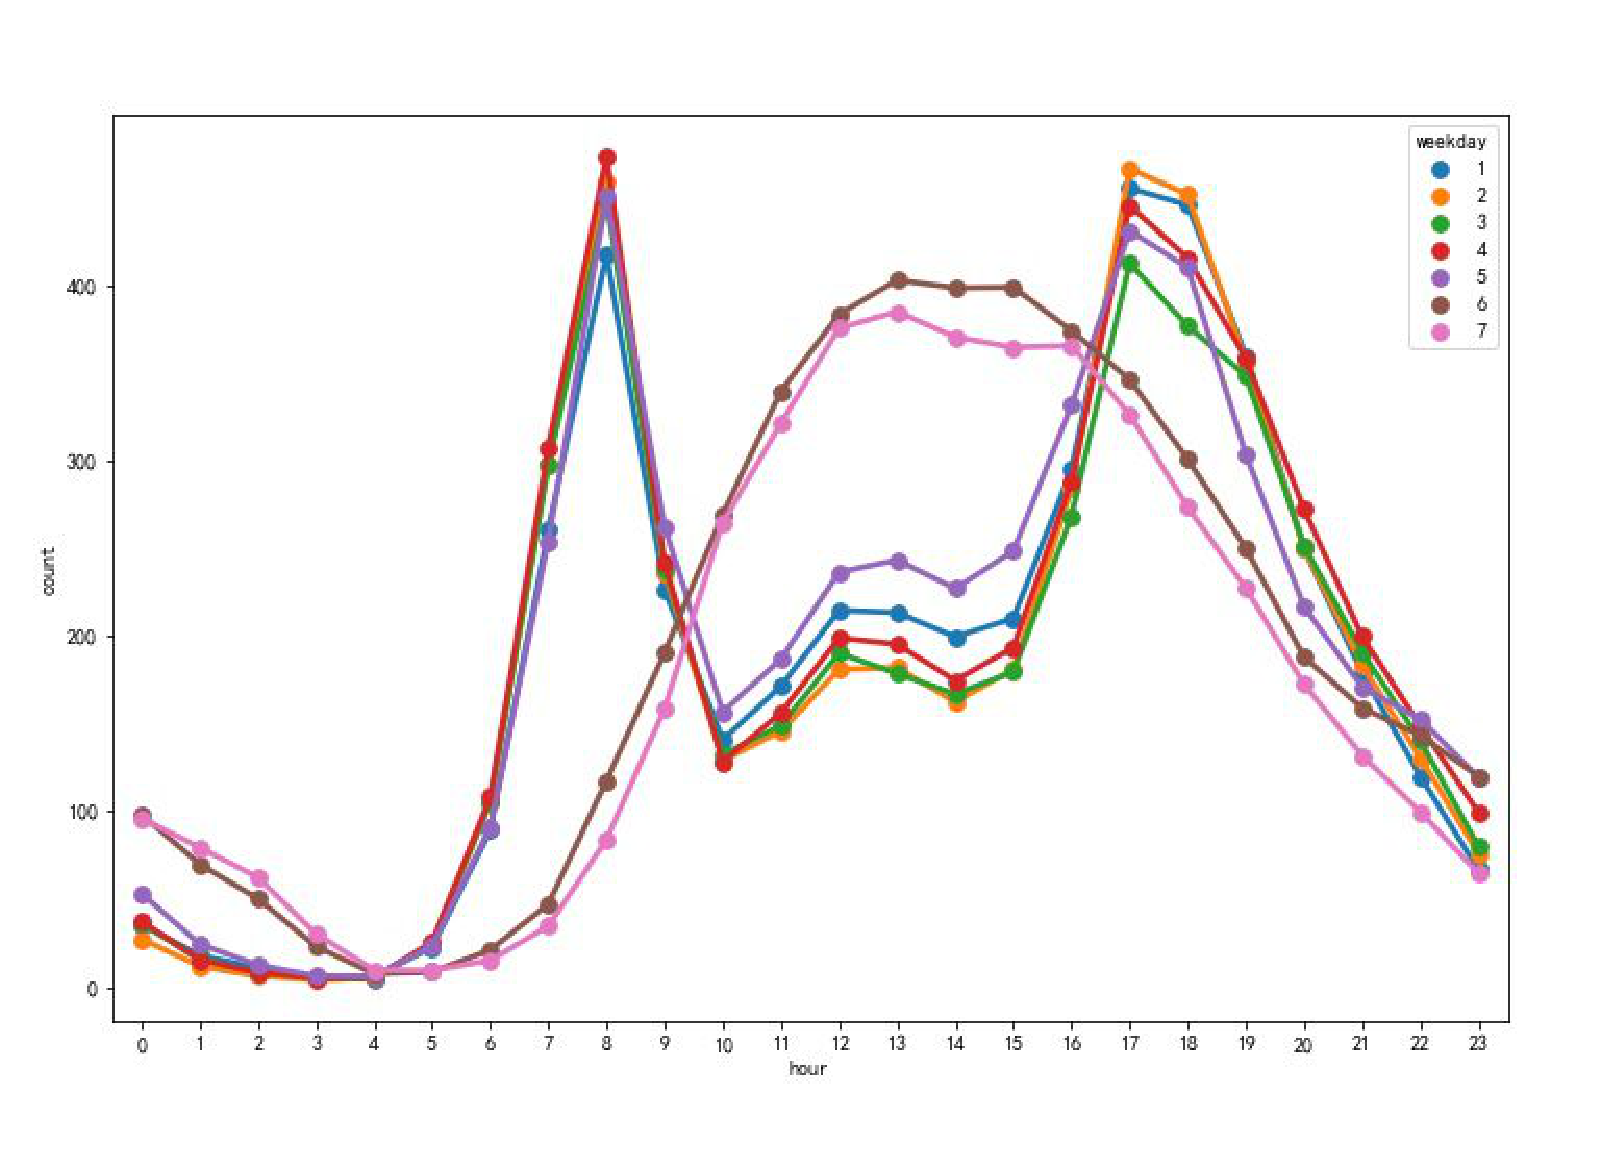
\includegraphics[width=0.4\textwidth]{pic/three hour2 (1).eps}
      \end{figure} 
     
    }
    \end{center}
 


\end{slide}
%%==========================================================================================
\begin{slide}[toc=,bm=]{Data  Visualization}
  \begin{center}

    {
      \begin{itemize}
        
          \item Draw the thermal diagram of the correlation coefficient
      \end{itemize} 
        \begin{figure}
          \centering
          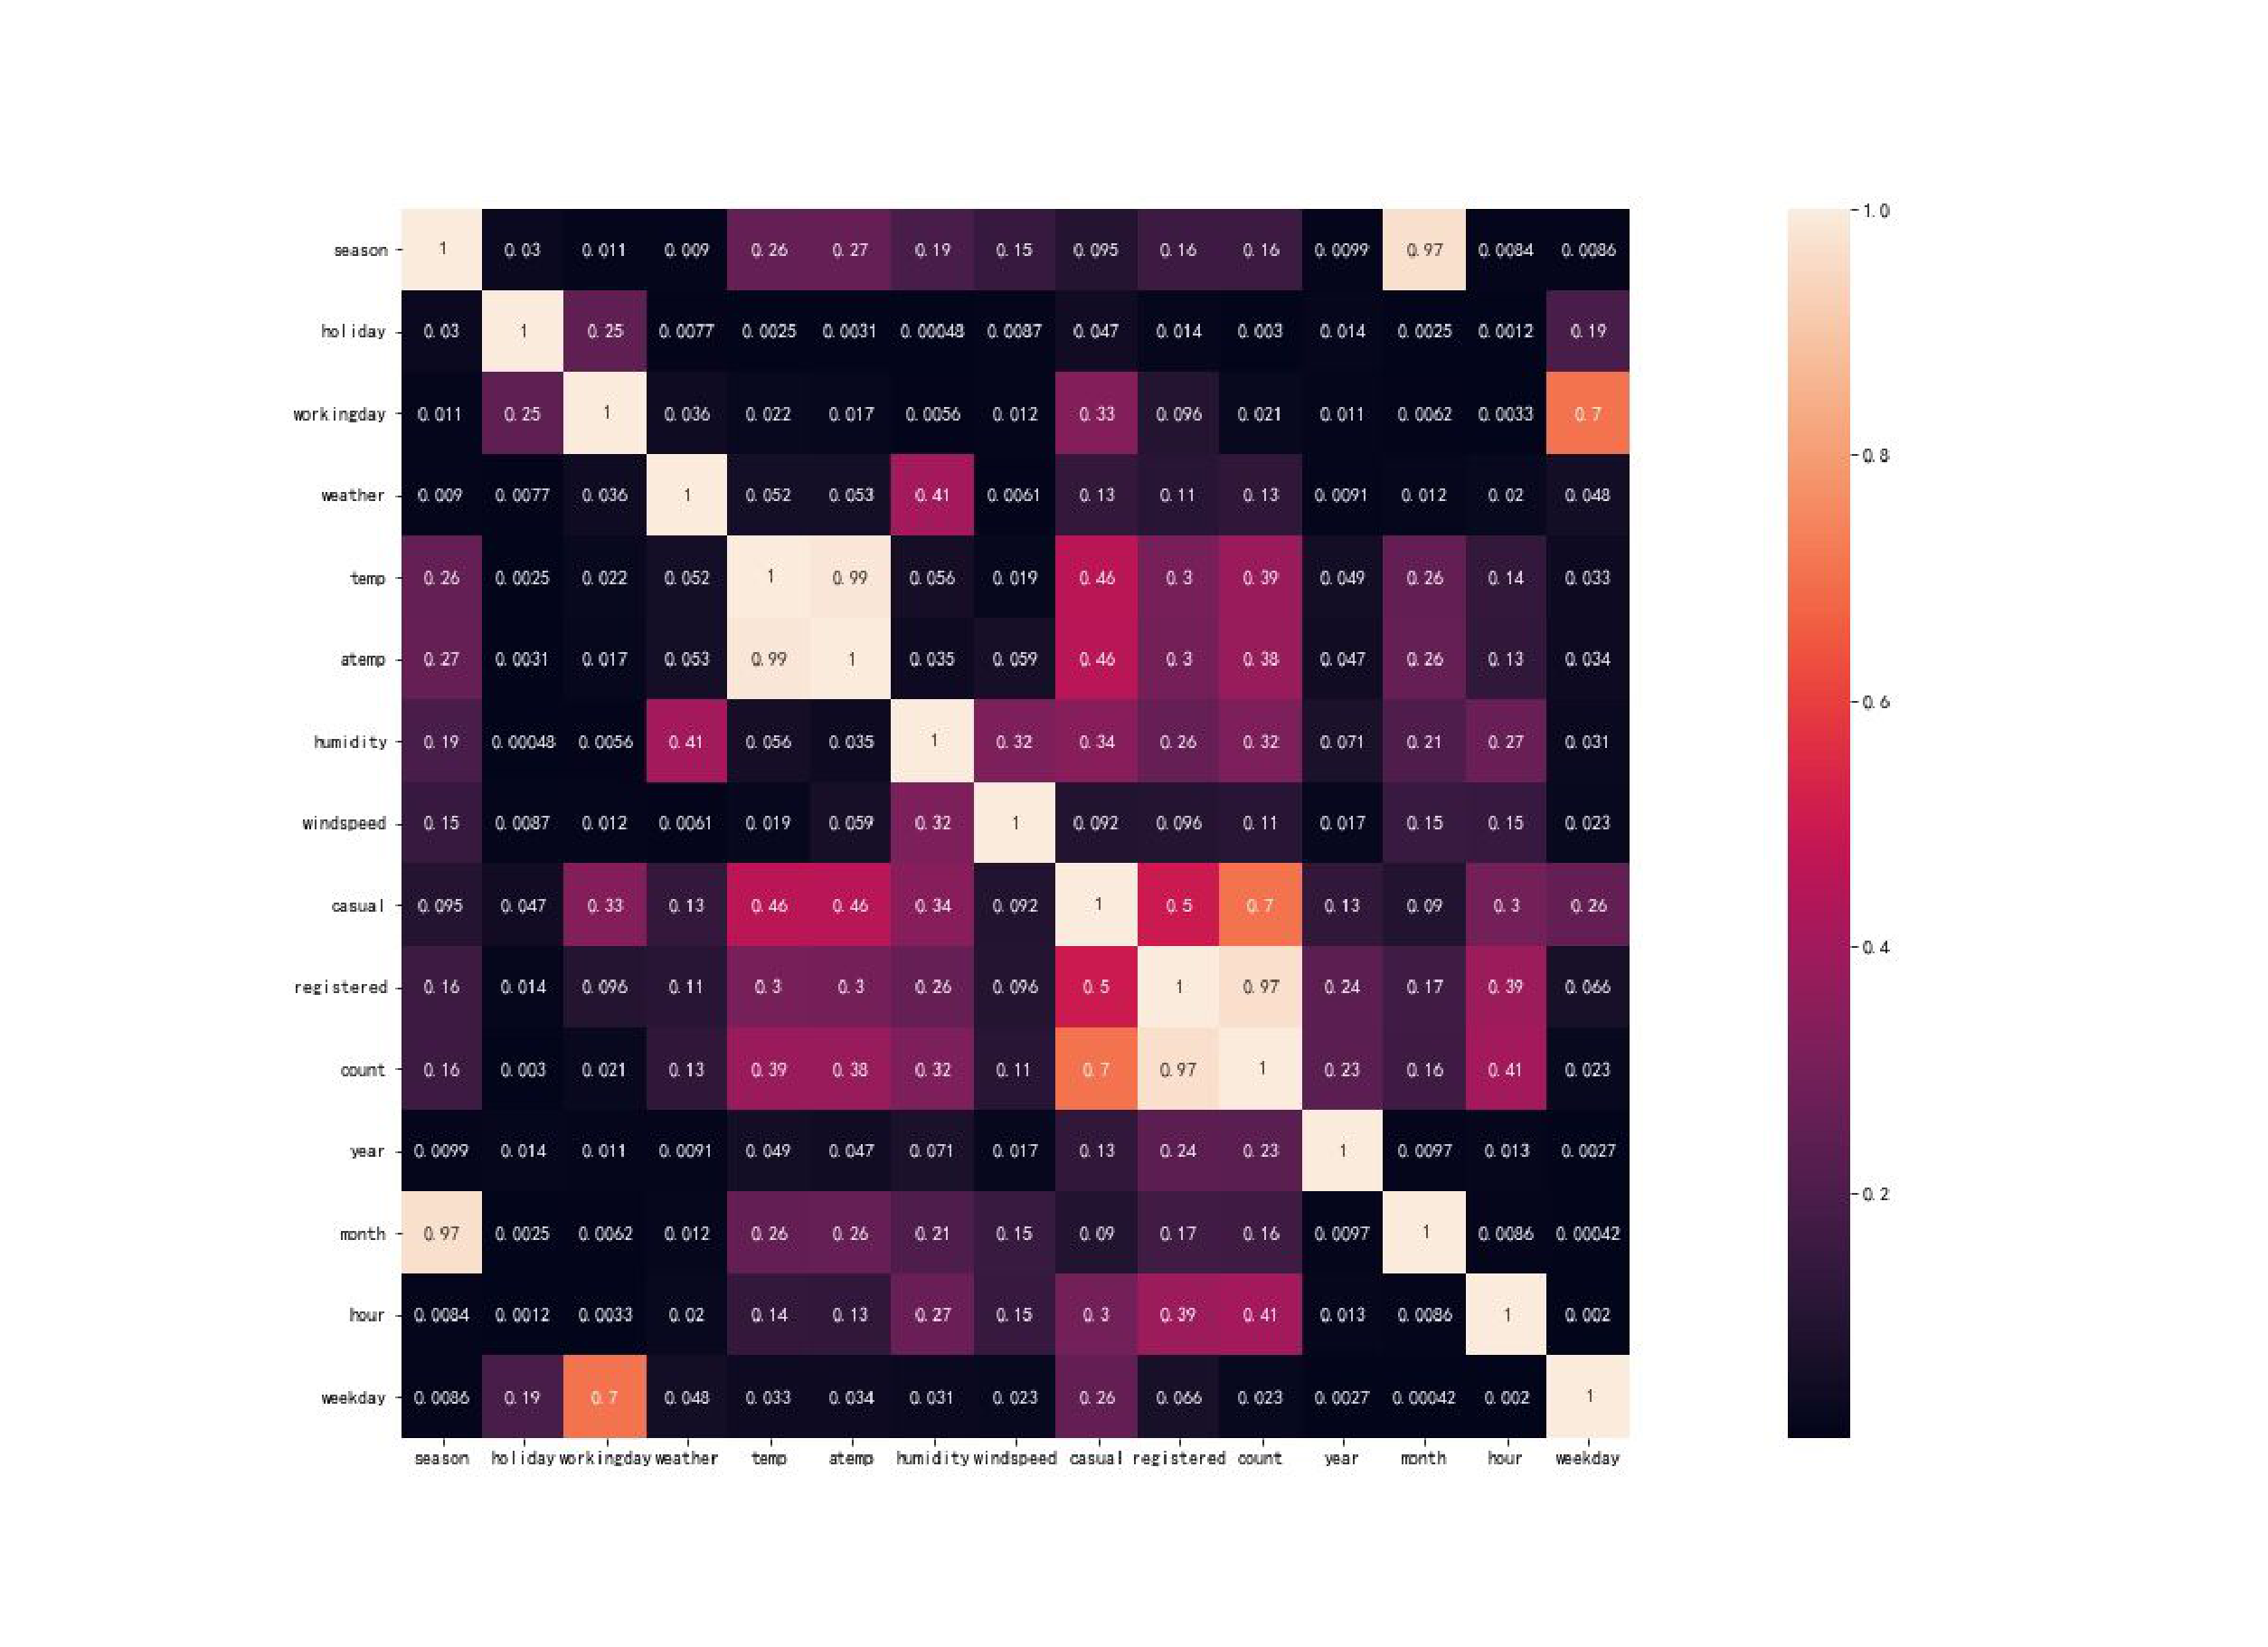
\includegraphics[height=0.5\textwidth]{pic/hot (1).eps}
          \centering
        \end{figure} 
    }
    \end{center}
 


\end{slide}
%%
%%==========================================================================================
\begin{slide}[toc=,bm=]{Conclution}
  \begin{center}

    {
      \begin{itemize}
        
          \item Draw the thermal diagram of the correlation coefficient
      \end{itemize} 
        
    }
    \end{center}
 


\end{slide}
%%
\end{document}

\endinput
